\documentclass[12pt]{article}
\usepackage[utf8]{inputenc}
\usepackage{graphicx}
\usepackage{wrapfig}
\usepackage[margin = 3cm]{geometry}
\usepackage[safeinputenc, maxnames=10, backend = biber, sorting=none, url = false, doi = false, isbn = false, citestyle = numeric-comp]{biblatex}
\AtEveryBibitem{\clearlist{language}}
\AtEveryBibitem{\clearfield{note}}
\AtEveryBibitem{\clearfield{month}}
\AtEveryBibitem{\clearfield{publisher}}
\addbibresource{references.bib}
\renewbibmacro{in:}{}
\usepackage{colortbl}

\usepackage{amsmath}
\usepackage{amsfonts}


\title{}


\begin{document}


\maketitle



\section{Replica computations}

\subsection{Replica symmetric ansatz}
\label{analysisRS}

To deal with the thermodynamics of disordered systems we can take advantage of a well-known technique borrowed from the spin-glass literature, the replica method.
We can then handle quantities disordered quantities and eventually obtain the free energy by means of the identity $-\beta F=\lim_{n \rightarrow 0} \frac{\ln \overline{{Z^n}}}{n} $.
The starting point is then the computation of the replicated partition function, namely
\begin{equation}
    \overline{Z^n} = \int \prod_{i, (ij)} d n_i^a d \alpha_{ij} \exp \left[-\sum_{(ij)} \frac{(\alpha_{ij} - \mu /S)^2}{2 \sigma^2/S} -\beta H(\lbrace n_i^a \rbrace) \right]
\end{equation}
where the overline denotes the average over the disorder, \emph{i.e.} the average over the Gaussian variables $\alpha_{ij}$. 
To perform the computation -- that will involve quadratic terms in the product of the species abundances -- we introduce the overlap matrix $Q_{ab}$ (with diagonal value $Q_{aa}$) and the external field $H_a$, where $(a, b)=1,...,\tilde{n}$ stand for two replicas of the same system, \emph{i.e.}:
\begin{equation}
Q_{ab}=\frac{1}{S} \sum \limits_{i=1}^{S}  n_i^ a n_i^b \ , \hspace{1cm}
    H_a=\frac{1}{S} \sum \limits_{i=1}^{S}  n_i^a  \ .
\end{equation}
The free energy in the replica space turns out to be then
\begin{equation}
 F= -\frac{1}{\beta n}\ln \overline{\int \prod \limits_{a,(a<b)} d Q_{ab}d Q_{aa} d H_{a} \; e^{S \mathcal{A}(Q_{ab}, Q_{aa},H_a) }}
 \label{freeenergy_RS}
\end{equation}
where
\begin{equation}
\begin{split}
& \mathcal{A}(Q_{ab},Q_{aa},H_a)=  - \sigma^2 \beta^2 \sum \limits_{a<b}\frac{Q_{ab}^2}{2}-\sigma^2 \beta^2 \sum \limits_a \frac{Q_{aa}^2}{4}+ \mu \beta \sum_a \frac{H_a^2}{2}+\frac{1}{S}\sum \limits_i \ln Z_i \ .
\end{split}
\end{equation}
The last term above, the partition function $Z_i$, is
\begin{equation}
Z_i= \int \prod \limits_a d N_i^a \exp \left(-\beta H_\text{eff}(\lbrace n^a \rbrace_i ) \right) \ ,
\end{equation}
which depends on the effective Hamiltonian $H_{\text{eff}}$ as
\begin{equation}
\begin{split}
 H_{\text{eff}}(\lbrace n^a \rbrace_i )=& -\beta  \sigma^2 \sum \limits_{a <b} n_i^a n_i^b Q_{ab}  -\beta  \sigma^2 \sum \limits_a (n_i^a)^2 \frac{Q_{aa}}{2} + \sum \limits_a  \mu H_a n_i^a  + V_i(n_i^a) \ .  
\end{split}
\end{equation}
The simplest scenario in the panorama of all possible replica computations is the so-called replica symmetric (RS) ansatz, which turns out to be correct as long as the free-energy landscape is characterized by only a single equilibrium. 
Any permutation of the replica indices does not affect the matrix structure. Otherwise dais, within the RS ansatz the permutation symmetry of the replicated Hamiltonian is respected.
The overlap matrix is thus parametrized by two values: the self-overlap between replicas inside the same state, $q_d$, and the inter-state overlap, $q_0$. The external field is assumed to be uniform, $\forall a$.
\begin{equation}
\begin{split}
& Q_{ab}= q_0 \hspace{0.7cm }\text{if} \hspace{0.6cm} a \neq b    \\
& Q_{aa}=q_d \hspace{0.7cm }\text{if} \hspace{0.6cm} a = b\\
& H_a=h  \hspace{1.8cm } \forall a
\label{Ansatz_RS}
\end{split}
\end{equation}
The action $\mathcal{A}$ then becomes
\begin{equation}
\begin{split}
    \mathcal{A}(q_d,q_0,h)= & - \sigma^2 \beta^2 \frac{\tilde{n}(\tilde{n}-1)}{4} q_0^2 -\sigma^2 \beta^2 \frac{\tilde{n}}{4} q_d^2  +  \mu \beta \frac{\tilde{n}}{2} h^2 +\frac{1}{S} \sum \limits_{i} \ln Z_i 
    \end{split}
    \label{actionRS}
\end{equation}
where the partition function is integrated over $n_i^a$ with an effective Hamiltonian that depends now on the parameters $(q_d,q_0,h)$. 
Replica indices are nevertheless still coupled. 
At this stage, the replica trick comes into play allowing us to decouple replicas by the introduction of an auxiliary Gaussian variable $z$, with zero mean and unit variance, which makes the expression of the partition function of the form:
\begin{equation}
    Z_i= \int_{-\infty}^{+\infty} \frac{d z_i}{\sqrt{2 \pi}} e^{-z_i^2/2} \int \prod \limits_{a=1}^{\tilde{n}} d n_i^a e^{-\beta \sum \limits_a H_\text{RS}(n_i^a, z_i) } \ ,
\end{equation}
which is written in terms of the RS Hamiltonian:
\begin{equation}
\begin{split}
    H_\text{RS}(n_i,z_i)=& - \sigma^2 \beta (q_d-q_0) \frac{n_i^2}{2} +( \mu h - z_i \sigma \sqrt{q_0})n_i +V_i(n_i)=\\
    =&\frac{n_i^2}{2} \left[1-\beta \sigma^2(q_d-q_0) \right] -\frac{4}{3} n_i^{3/4}+(\mu h-z_i \sigma \sqrt{q_0})n_i
   \end{split} 
\end{equation}
where we recall that $V_i(n_i)=-\frac{4}{3} n_i^{3/4} +\frac{n_i^2}{2}$. 
In the thermodynamic limit, we can safely resort to the Laplace method that allows us by the minimization of the action $\mathcal{A}(q_d,q_0,h)$ to get the corresponding equations for the order parameters $(q_d,q_0,h)$.
\begin{equation}
\begin{split}
& q_d= \int \mathcal{D} z \left(\frac{ \int_{0}^{n^{\text{up}}} d n e^{-\beta H_{\text{RS}}(q_0,q_d,h,z)} n^2}{ \int_{0}^{n^{\text{up}}} d n e^{-\beta H_{\text{RS}}(q_0,q_d,h,z)}} \right) = \overline{\langle  n^2 \rangle} \ , \\ 
& q_0= \int \mathcal{D} z \left(\frac{ \int_{0}^{n^{\text{up}}} d n e^{-\beta H_{\text{RS}}(q_0,q_d,h,z)} n}{ \int_{0}^{n^{\text{up}}} d n e^{-\beta H_{\text{RS}}(q_0,q_d,h,z)}} \right)^2  = \overline{ \langle n \rangle^2}  \ , \\ 
& h= \int \mathcal{D} z \frac{ \int_{0}^{n^{\text{up}}} e^{-\beta H_{\text{RS}}(q_0,q_d,h,z)} n}{ \int_{0}^{n^{\text{up}}} d n e^{-\beta H_{\text{RS}}(q_0,q_d,h,z)}}=\overline{ \langle  n \rangle} \ .
\label{equations_SP}
\end{split}
\end{equation}
The calligraphic notation stands for the Gaussian integral $\mathcal{D}z \equiv \int \frac{dz}{\sqrt{2 \pi}} e^{-z^2/2}$. More precisely, the most internal average corresponds to the standard average over the Boltzmann measure, while the external one denotes the average over the quenched disorder. The quenched disorder is indeed modelled via the introduction of an auxiliary Gaussian variable in order to decouple replicas. 
The solution of such equations can be studied iteratively: to perform the numerical integration, we choose the upper bound of the integral over the abundances as $N^{up}=100$ and a damping parameter $\alpha=0.1$.


\subsection{Stability analysis}

The replica symmetric solution presented thus far is correct unless the energy landscape remains purely convex, namely only if (minus) the action in Eq. (\ref{actionRS} admits a unique minimum. To properly figure out this condition, we need to compute the harmonic fluctuations around the RS solution and study their stability. Once the expression of the stability matrix is available, \emph{i.e.} the matrix of second derivatives of the action w.r.t $Q_{ab}$, we diagonalize it on a suitable sector, called \emph{replicon subspace}, and eventually obtain the first vanishing eigenvalue. 
Within the RS approximation, the replicon reads:
\begin{equation}
\lambda_R \propto \left[ 1-(\beta \sigma)^2 \overline {\left( \langle n^2 \rangle -\langle n \rangle^2 \right)^2} \right]
\end{equation}
whose vanishing behavior corresponds to an unstable single equilibrium phase and signals the emergence of critical behavior.

From what discussed above, we should expect the system to remain significantly more stable at rather high values of $\sigma$, in particular at those values at which a phase transition occurred in the basic LV model. We thus analyze the resulting phase diagram in the very high $\beta$ regime when the production term, either linear or logistic in classical models, is replaced by $N^{3/4}$. 
nBy the computation of the smallest eigenvalue of the stability matrix, we claim that the transition to the multiple equilibra phase is shifted to much higher $\sigma$ values at variance with the ordinary Lotka-Volterra model (in the $\beta \rightarrow \infty$ limit it occurs at $\sigma_c=1/\sqrt{2}$. See \cite{Biroli2018, Altieri_PRL2021} for a clearer picture).


\section{Analysis with different carrying capacities}

,In the following, we shall discuss the general case of non-unitary carrying capacities rephrasing what we have done in Sec. \ref{analysisRS} with the following one-species potential:
\begin{equation}
  V_i(n_i)= -\frac{4}{3} n_i^{\frac{3}{4}} +\frac{n_i^2}{2 K^{\frac{5}{4}}} \ .
\end{equation}
As pointed out in the text, in the limit of infinite $K$ we expect the transition line to be dramatically pushed down. The single stable phase will be then reduced upon increasing $K$ persisting only for very small $\sigma$.
In other words, choosing only small values of $\sigma$ and high $\mu$ corresponds to peaking the distribution around interaction values $\alpha_{ij}$ that are strictly positive. 

\begin{figure}[h]
    \centering
    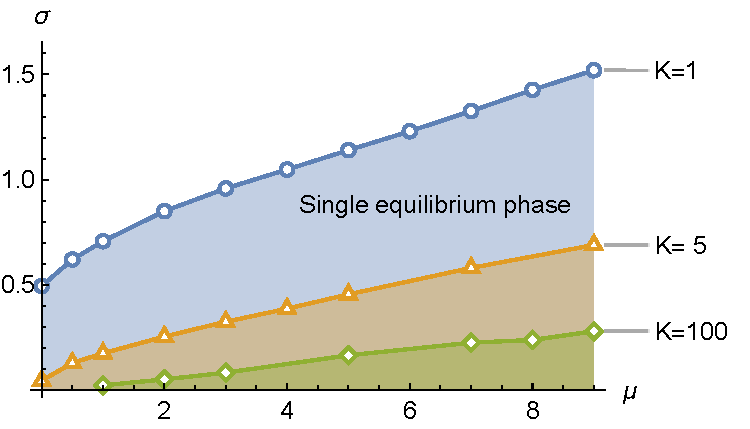
\includegraphics{phased_complete.pdf}
    \caption{Phase diagram showing the heterogeneity parameter $\sigma$ as a function of the average interaction $\mu$ for different values of the carrying capacities, $K=1$ in blue, $K=5$ in orange, and $K=100$ in light green. The coloured phases show the presence of a single equilibrium for the species pool, whereas beyond the transition lines the solution becomes marginal and no longer converges to a single stable fixed point.}
    \label{phasediagram_K}
\end{figure}


\section{Functional response}

To better probe the stability properties of each phase, we can focus on the density of eigenvalues within a Random Matrix Theory approach. 
The density of eigenvalues $\lambda_\gamma$ is
\begin{equation}
\rho(E)= \frac{1}{S} \sum_{\gamma}\delta(E-\lambda_{\gamma})
\end{equation}
where $S$ stands for the number of species.
Its expression is strictly connected to the resolvent matrix $G(E)$ 
\begin{equation}
\rho(E)= \lim_{\epsilon \rightarrow 0^{+}} \frac{1}{\pi S} \Im \; {\text{Tr} \; G(E-i \epsilon)}
\label{density_E}
\end{equation}
where $\Im( \cdot )$ is the imaginary part. Therefore, the spectral properties can be obtained by rephrasing the problem in terms of the analysis of the resolvent matrix structure, which reads
\begin{equation}
G_{ij}(z)= \left (\frac{1}{z \mathbb{1}-H} \right)_{ij} ,
\end{equation}
$H$ being the Hessian matrix $H_{ij}=V^{''}(n^{*}_i)\delta_{ij}+\alpha_{ij}$. $V^{''}(n^{*}_i)$ is the curvature of the potential associated with the functional response of species $i$ evaluated at the abundance of this given species. 
Provided that the $\alpha_{ij}$s, the non-vanishing off-diagonal elements of the Hessian, satisfy a tree-like structure, the diagonal contribution of the resolvent can be written as
\begin{equation}
G_{ii}(z)=\frac{1}{z-V_{ii}^{''}-c \sum_{j \in \partial i}  \alpha_{ij}^2 G_{j \rightarrow i}(z)} \ .
\label{resolvent_diag}
\end{equation}
where we have split the diagonal from the non-diagonal counterpart at the denominator and rewritten the last term in the denominator as the contribution that the resolvent would get without the edge between $i$ and $j$, summed over $j$ for all $j$ in the neighbourhood of species $i$. The proportionality factor $c$ accounts for the number of surviving species and will be clarified later.

This formulation was first proposed in a completely different context by \cite{abou1973} but can be re-obtained in a straightforward way by using perturbation theory.
Since in the large-$S$ limit non-diagonal terms (with $k \neq j$) are negligible, we can stick on the diagonal counterpart only. To be more define, on every graph with a tree-like topology, sites $k$ and $j$ turn out to be directly connected once that $i$ is removed.
For the sake of brevity, we will denote the diagonal element of the resolvent matrix as $G(z)$ implying an equality in distribution for the two random variables at the l.h.s and the r.h.s..
%\begin{equation}
%G(z) \myeq \frac{1}{z-V^{''}(N^{*})-c \sum \limits_{l=1}^{k+1}\hat{G}_l(z)} \end{equation}
Written in a more compact form, it becomes:
\begin{equation}
G(z)=\biggl \langle \frac{1}{z-V^{''}(n^{*}) -\phi \sigma^2 G(z)} \biggr \rangle \  ,
\end{equation}
where $\phi=S^{*}/S$ accounts for the diversity, namely the ratio between the number of alive species and the total number in the pool (the prefactor $c$ in the previous notation).
The brackets denote the final average over the probability distribution $P(N^{*})$ as the local curvatures of the potential depend now on the abundance at the fixed point. 

The necessary condition for stability or marginal stability is associated with finite and infinitesimally small eigenvalues of the stability matrix, respectively. The smallest eigenvalue is indeed proportional to the left edge of the support of the spectral density $\rho(\lambda)$. 
To identify the leading behavior of the distribution of eigenvalues close to the transition we need to find the condition for the lower edge of the spectrum, $\lambda_0$ precisely happening at $G=G_0$:
\begin{equation}
G(\lambda_0)=\biggl \langle \frac{1}{\lambda_0-V^{''}(n^{*}) -\phi \sigma^2 G(\lambda_0)} \biggr \rangle \  ,
\end{equation}
We perform then a $\lambda$-expansion in the equation for the imaginary part of the resolvent eventually finding at $\lambda_0=0$ 
\begin{equation}
1=\phi \sigma^2\biggl \langle \left(\frac{1}{(V^{''}(n^{*}) +\phi \sigma^2 G(\lambda)} \right)^2\biggr \rangle
\end{equation}
This condition implies in terms of the smallest (replicon) eigenvalue:
\begin{equation}
\lambda_R=1-\phi \sigma^2 \biggl \langle \frac{1}{(V^{''}(n^{*}) +\phi \sigma^2 G(\lambda))^2}  \biggr \rangle=1-\phi \sigma^2 \int {\frac{dP(n^{*})}{(V^{''}(n^{*}) +\phi \sigma^2 G(\lambda))^2}} \ .
\end{equation}

According to our definition of the potential in Eq. (\ref{quadratic_potential}), the functional response is now species-dependent with $V^{''}(n)=1+\frac{1}{4} n^{-5/4}$, to be eventually averaged over the distribution $P(n^{*})$. Therefore, in the limit of very small abundances, $V^{''}(n^{*})$ would get a diverging contribution from the second term, which nonetheless does not result in a divergent behavior of the integral evaluated in its lower extreme. For small abundances, the solution remains stable with $\lambda_R$ positive. Diverging solutions can arise in the opposite limit, at very large $n^{*}$.


\printbibliography
\end{document}


